\documentclass{article}

\usepackage[utf8]{inputenc}
\usepackage[portuguese]{babel}
\usepackage{blindtext}
\usepackage{graphicx}
\usepackage{amsmath}
\usepackage{float}
\usepackage{caption}
\usepackage[compact]{titlesec}
\usepackage{multicol}
\usepackage[a4paper, total={7.5in, 10in}]{geometry}
\usepackage[font=scriptsize,labelfont=bf]{caption}
\usepackage{listings}
\usepackage{color}
 
\definecolor{codegreen}{rgb}{0,0.6,0}
\definecolor{codegray}{rgb}{0.5,0.5,0.5}
\definecolor{codepurple}{rgb}{0.58,0,0.82}
\definecolor{backcolour}{rgb}{0.95,0.95,0.92}
 
\lstdefinestyle{mystyle}{
    backgroundcolor=\color{backcolour},   
    commentstyle=\color{codegreen},
    keywordstyle=\color{magenta},
    numberstyle=\tiny\color{codegray},
    stringstyle=\color{codepurple},
    basicstyle=\footnotesize,
    breakatwhitespace=false,         
    breaklines=true,                 
    captionpos=b,                    
    keepspaces=true,                 
    numbers=left,                    
    numbersep=5pt,                  
    showspaces=false,                
    showstringspaces=false,
    showtabs=false,                  
    tabsize=2
}
 
\lstset{style=mystyle}

\setlength{\columnsep}{1cm}
\setlength{\parindent}{0em}
\titlespacing{\section}{1pt}{*0.5}{*0.5}
\begin{document}

\textbf{Relatório de Entrega de Trabalho} \newline
\textbf{Disciplina de Programação Paralela (PP)}\textbf{ - Prof. César De Rose} \newline
\textbf{Alunos:} Rafael Rios e Rodrigo Silveira \newline
\textbf{Exercício:} TPD2: Algoritmos Distribuídos de Eleição (MPI) \newline

\begin{multicols*}{2}

\section{Modelagem utilizada}
A fim de avaliar a execução de um algoritmo de distribuição por eleição, usou-se a biblioteca MPI (Message Passing Interface), a qual implementa diversas funções que compreendem um padrão para comunicação de dados em computação paralela, para desenvolver a modelagem de um anel lógico para 'n' processos. Desta forma, o anel deve trocar mensagens apenas com o próximo nodo seguinte a ele, onde o processo de maior índice corresponde ao coordenador. O sistema de eleição é proposto quando o coordenador falha, neste caso, um dos processos deve avisar os demais que uma eleição para a escolha do próximo coordenador ocorrerá. \newline

\section{Implementação}
O algoritmo implementado primeiramente escolhe de maneira aleatória qual o processo detectará a falha, esta escolha é realizada pelo processo 0, o qual propaga a informação para o restante do anel, deste modo, é garantida a sincronização da execução, como pode ser visto na Figura 1. 

\begin{figure}[H]
            \centering
            \vspace{-0.3em}
            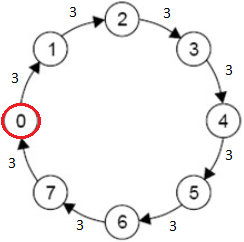
\includegraphics[width=4cm, height=4cm]{anel_falha.png}
            \vspace{-0.6em}
            \caption{Anel lógico para 8 processos - Detecção de falha}
            \vspace{-1.1em}
\end{figure}

No segundo momento, fica a cargo do processo escolhido para detectar a falha começar a eleição (processo 3 no exemplo), transmitindo pelo anel a mensagem com o vetor para cada processo cadastrar o seu respectivo índice, sendo a primeira posição do vetor responsável por guardar o próximo índice do vetor a ser escrito (Figura 2).

\begin{figure}[H]
            \centering
            \vspace{-0.3em}
            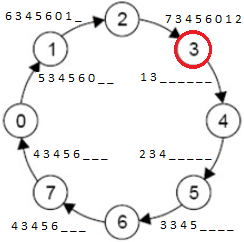
\includegraphics[width=4cm, height=4cm]{anel_eleicao2.png}
            \vspace{-0.6em}
            \caption{Anel lógico para 8 processos - Eleição}
            \vspace{-1.1em}
\end{figure}

Com isso, ao retornar para o processo que começou a eleição, é realizada a escolha do próximo coordenador,  sendo escolhido o processo com o maior índice cadastrado no vetor propagado (processo 6), por fim, a mensagem com o índice do processo coordenador é transmitida, para que todos processos saibam quem é o atual eleito.

\begin{figure}[H]
            \centering
            \vspace{-0.3em}
            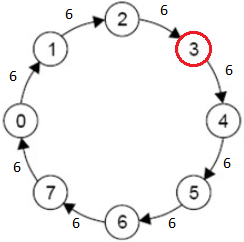
\includegraphics[width=4cm, height=4cm]{anel_coordenador.png}
            \vspace{-0.6em}
            \caption{Anel lógico para 8 processos - Escolha do coordenador}
            \vspace{-1.1em}
\end{figure}

\section{Dificuldades encontradas}
Entendimento da biblioteca MPI e o seu funcionamento ao encadear processos através da lógica de "Send" e "Receive"; Desenvolvimento da lógica para avisar a todos os processos qual será o escolhido para detectar a falha, pois caso fosse chamada a função rand() para todos os processos, haveria uma dessincronização entre os mesmos, caracterizando um erro ao propagar-se a informação para todos os outros processos. \newline

\section{Testes}
Foram executados testes para diversos números de processos diferentes, visando observar possíveis falhas e mudanças no desempenho, entretanto, para todas as execuções obteve-se o mesmo resultado esperado, como também, o mesmo desempenho. \newline

\section{Observações Finais}
A implementação realizada se mostrou viável para qualquer quantidade de processos, tendo sua lógica baseada nos algoritmos desenvolvidos e propostos em sala de aula, tornando de grande importância o entendimento da biblioteca MPI para a execução de programas computacionais paralelos, como também, para o decorrer dos desenvolvimentos propostos, tornando possível compreender diversos aspectos teóricos que foram abordados na disciplina.

\end{multicols*}

\newpage

\lstinputlisting[language=C++]{pipe_basico.c}

\newpage

\begin{figure}[H]
            \centering
            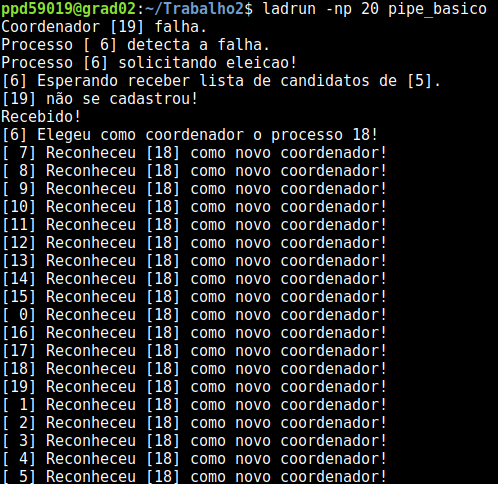
\includegraphics[width=13cm, height=12cm]{exemplo_saida.png}
            \caption{Output para 20 processos}
\end{figure}

\begin{figure}[H]
            \centering
            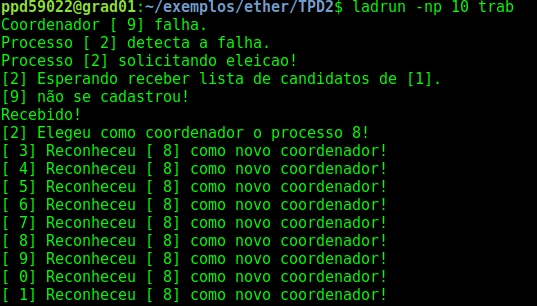
\includegraphics[width=13cm, height=8cm]{ex_10.png}
            \caption{Output para 10 processos}
\end{figure}

\end{document}
